\section{Word2Vec Model}

\subsection{Word Embedding Representations: Count-Based vs. Context-Based}
 
Word embeddings are generally learned via two kinds of vector space models, both using contextual knowledge: 

Count-based vector space models are unsupervised learning algorithms based on matrix factorization of a global word co-occurrence matrix. The main assumption is that words in similar contexts share related semantic meanings. Examples include PCA and neural probabilistic language models. Another term for this type is \emph{distributed semantic model} (DSM).

Context-based vector space models are supervised algorithms that use a local context to predict target words. These are predictive models which take dense word vectors as parameters and update word representations during training.

In 2014, Baroni et al. showed that predictive approaches outperformed count models significantly and consistently. 

Algorithms like Word2Vec and GloVe are considered predictive and context-based vector space models, although they also rely on co-occurrence counts. 

Word2Vec is an unsupervised learning algorithm for obtaining word vector representations using a two-layer neural network. Its input is the text corpus and output is the set of feature vectors, as one vector per word. Generally, Word2Vec learns words similarities, thus allowing mathematical operations to be done on word vectors. There are two main models part of Word2Vec: the Skip-gram and Continuous Bag of Words (CBOW) algorithms. 

\subsection{Skip-Gram Model}

\subsubsection{Motivating the Skip-Gram Model}

Existing word representations already capture linguistic patterns, allowing algebraic operations to be done on the word vectors in their semantic vector space; for example, $vector(\textit{"King"}) - vector(\textit{"Man"}) + vector(\textit{"Woman"})$ outputs a vector close to the word vector for ``Queen".

Mikolov et al. (2013b) created the Skip-Gram to learn word vector representations from large data sets in an efficient manner. Previous architectures were trained with much fewer words and smaller word vector dimensionality, thus reducing the quality of learned representations. 

\subsubsection{Defining the Skip-Gram Model}

A key concept for what follows is \textbf{one-hot vector encoding}. A one-hot encoding is the simplest form a word embedding where there is one cell for each vocabulary word, so its dimension equals the vocabulary size. A $1$ is placed in the cell marking the position of the word in the vocabulary, and a $0$ is placed in all other cells. However, this can result in high-dimensionality vector representations for large vocabularies, resulting in high computational costs, and similarity between categories cannot be represented. 

The Skip-Gram model uses a fixed sliding window $c$, or size of the training context to capture context along a sentence. A target word thus has left and right context words within that sliding window. This centre word is represented using a \emph{one-hot} encoded vector that is passed to a neural network which updates the vector to have high (values close to $1$) in cells corresponding to predicted context words. 

Consider the following example of target and context pair words as training samples, using context window size $c = 5$. 

\begin{figure}[h]
\centering
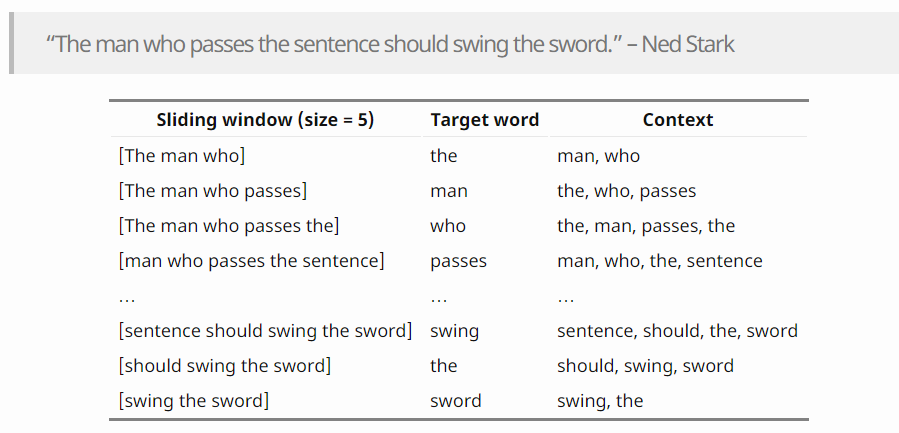
\includegraphics[width=0.7\textwidth]{imgs/skipgram_quote.png}
\caption{Sliding Window Demonstration for Skip-Gram. From \emph{Learning Word Embeddings}, by Lilian Weng, 2017. \url{https://lilianweng.github.io/lil-log/2017/10/15/learning-word-embedding.html}. Copyright n.d. by n.d.}
\end{figure}

For case of target word ``swing", the four context words are used to create four training samples: (``swing", ``sentence"), (``swing", ``should"), (``swing", ``the"), and (``swing", ``sword"). 

The Skip-Gram is illustrated below. The input vector $\overrightarrow{x} = (x_1,..., x_V)$ and output vector $\overrightarrow{y} = (y_1,...,y_V)$ are both one-hot encoded word representations, and the hidden layer of the neural network representation is a word embedding with dimension $N$. (Thus even though the vocabulary size is $V$, the goal is to learn embeddings with size $N$). Overall, the model predicts one context word, the output $\overrightarrow{y}$, given one target word, the input $\overrightarrow{x}$, at a time: 

\begin{figure}[h]
\centering
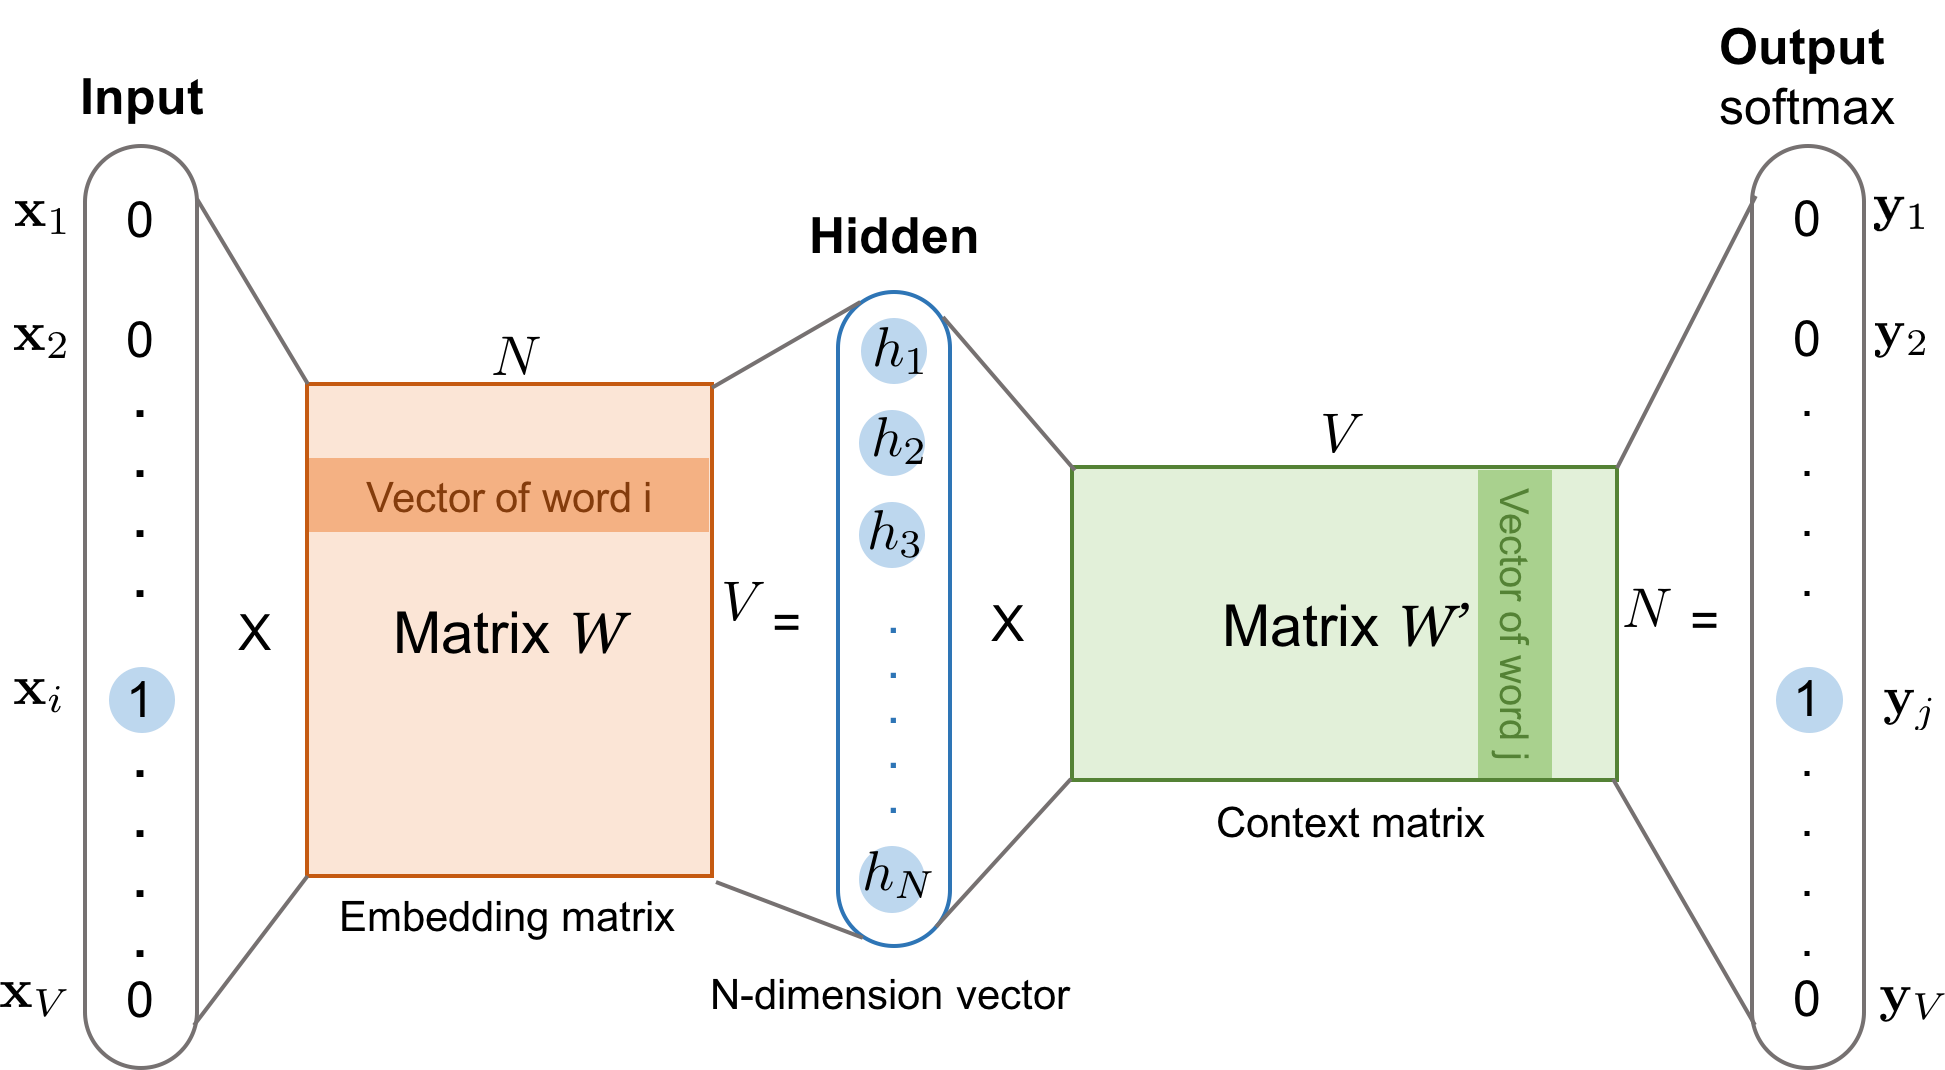
\includegraphics[width=0.6\textwidth]{imgs/skipgram_image.png}
\caption{Skip-Gram Model, with one target word vector as input. From \emph{Learning Word Embeddings}, by Lilian Weng, 2017. \url{https://lilianweng.github.io/lil-log/2017/10/15/learning-word-embedding.html}. Copyright n.d. by n.d.}
\end{figure}

The procedure for learning word vectors is: 

1. the input target word $w_i$ and output context word $w_j$ are encoded as one-hot vectors, $\overrightarrow{x}$ and $\overrightarrow{y}$.

2. A randomly initialized word embedding matrix $W$ with size $V \times N$ is multiplied with $\overrightarrow{x}$ to give the $N$-dimensional embedding for target word $w_i$. This embedding resides in the $i$-th row of $W$ and also is part of the hidden layer of the model. 

3. Next, the hidden layer is multiplied by a word context matrix $W'$ with size $N \times V$ to produce the one-hot encoded context vector, $\overrightarrow{y}$. \textbf{NOTE: }the output context matrix $W'$ encodes words as context and is distinct from the embedding matrix $W$. 

Mikolov et al. (2013a) defines the loss function to find word representations to predict context words of a target word: given the training word sequence $w_1, w_2, ..., w_T$ with $T$ training samples, the Skip-Gram maximizes the average log probability
$$
\frac{1}{T} \sum_{t=1}^T \sum_{-c \leq j \leq c, j \neq 0} log (P(w_{t+j} \;| \; w_t))
$$
where $c =$ the training size context window. 

For computing the probability of a surrounding word $w_{t+j}$ given the target centre word $w_t$,
$$
P \Big(w_{t+j} \; | \; w_t \Big) = \frac{ \exp{} } {}
$$

$$
P(w_t \; | \; w_{t-1}, ..., w_{t-n+1}) = \frac {\exp{ \Big(h^T \cdot v_{w_t}' \Big) }} {\sum_{w_i \in V} \exp{ \Big(h^T \cdot v_{w_i}' \Big) }}
$$










\subsubsection{Phrase-Learning Approach Using Skip-Gram Model}

Mikolov et al. (2013a) state that a problem with previous word vectors is their lack of phrase representation - the phrases ``Canada" and ``Air" could not be recognized as part of a larger concept and thus combined into ``Air Canada". 

Thus, Mikolov et al. (2013a) updated the Skip-gram to learn distributed representations of words and phrases that capture semantic and syntactic word relationships and that exhibit a linear structure that makes analogical reasoning possible in a vector space. 

TODO ... describe KEY FEATURE OF LOSS FUNCTION and volga river and berline examples

\subsection{Continuous Bag of Words Model (CBOW)}